\section{Discussion}

We find difficulty overcoming basic baselines in the competition.
In particular, frequency-based baseline submissions can be significantly more effective than the solutions proposed in our research of the problem.
These solutions are done by predicting the top 25 species at varying levels of locality (e.g., globally or regionally) and by dataset.
However, we find that latitude and longitude are surprisingly predictive of plant species in the dataset given an appropriate loss function.
Using these geospatial features provides a useful diagnostic for more complex datasets, since the number of input features are small and are easier to debug.
One possible limitation of our methodology is that we do not utilize the presence-only dataset with the exception of pre-training the tile2vec model.

\subsection{Alternatives Methods}

Learning a relationship between latitude and longitude to species labels with classical machine learning techniques and standard libraries is computationally intractable.
We note alternative approaches that were explored but did not produce results for various reasons.

\subsubsection{Classical Supervised Learning}

Intead of using a neural network to learn a mapping from location to species, we tried learning the mapping via logistic regression.
This numerically simple model can be learned using Spark via stochastic gradient descent (SGD). 
As a validation, we build a model to predict the 10 most frequent species in the dataset per site using only the location features. 
This achieves an F1-macro score of 0.09 when splitting the sites into a 90-10 train-validation split, which is better than random but roughly equivalent to always choosing the most frequent species.

We run into out-of-memory (OOM) issues when learning 5 million rows and 10,358 species with scikit-learn or statsmodels.
When we run the same procedure in Spark via distributed stochastic gradient descent (SGD), we find it will run for over 48 hours on a GCP n1-standard-8 instance (8 vCPU, 16GB RAM, 350GB NVME SSD) using 3-fold cross-validation (CV). 
We suspect that this is due to the size of the coefficients that involve J features and K output classes. 
Presuming an 8-byte double, the coefficients alone will be at least 8MB, larger than the typical CPU cache. 

We investigate other algorithms for modeling multilabel classification, including Naive Bayes, SVM, Random Forests, and Factorization Machines.
Naive Bayes assumes non-negative count data. 
SVMs are not tractable for our problem and are slower to solve than linear/logistic regression for other problems in the Spark toolbox. 
Random forests only support up to 100 classes in Spark, likely due to the branching factor to support each class. 
Factorization machines suffer from a similar issue as logistic regression and SVMs. 
Our final attempt to model multi-class classification via classical supervised techniques is through XGBoost \cite{chen2016xgboost}, which maintains a Spark binding. 
We run out of memory when trying to model many classes. 


\subsubsection{Low-rank Multilabel-Space Regression}

Instead of trying to learn the mapping between features and label-space directly, it is possible to learn a relationship between features and a low-rank multi-label space instead \cite{dasgupta2023review}.
It takes 30 minutes to learn a regression between location and a single binary response using either linear regression or XGBoost.
Given these constraints, we would like to constrain our model to 4-8 response variables. 

We try reducing the label space via the DCT since the relationship is trivially invertible in the machine learning pipeline. 
We find that this is untenable since we need many more coefficients than are available in our budget to represent discontinuities in species presence.
% Due to a bug in our initial exploration of a sparse label space (and a lack of deep thought into the approach), we implement the entire pipeline to find that we cannot use a thresholding approach to quantize the results of the reconstructed label space.

% \begin{figure}
%     \centering
%     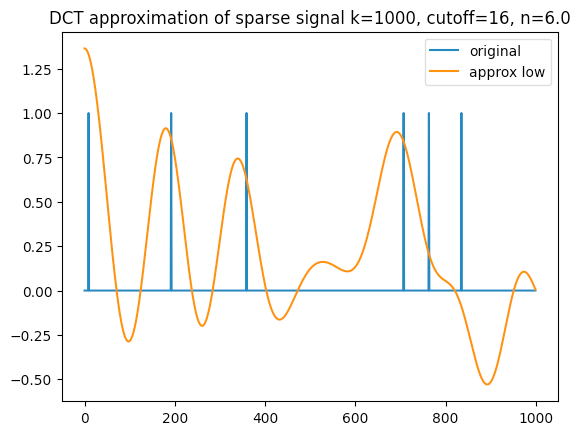
\includegraphics[width=0.7\textwidth]{figures/label-dct-sparse.png}
%     \caption{DCT of the label-space using the first 16 components.}
%     \label{fig:label-dct-sparse}
% \end{figure}

Another approach is to use singular value decomposition (SVD) to compute a projection of label-space into the first few eigenvectors, and then learn the relationship between the features and the projection \cite{tai2012multilabel}.
Then, predictions are quantized using nearest neighbors in the projection of the label space.
This process is similar to latent semantic indexing (LSI), and would allow a model to take into consideration cooccurrences between labels. 
While interesting, this approach requires significant engineering effort for results that are no more interpretable than neural networks.

\subsubsection{Node2Vec}

Node2vec \cite{grover2016node2vec} learns to preserve properties of network nodes using biased random walks.
Using the K-NN graph, we attempt embedding the survey sites using the co-occurrences of species among sites.
We could then use the embedding of the survey site as a feature for the classification task.
The embedding of the survey node is intractable due to the size of the network of 4 million nodes and ~1 billion edges. 
A species node embedding can be computed in 20 minutes, which results in a vector representation of species that can be used for clustering or classification.

A survey node embedding would be useful as a feature of the classification task since it would require no further processing to go from the survey site to the species. 
To take advantage of the species embeddings, we would need to compute some average of the embedding vectors before passing into a supervised classification model.

\section{Future Work}

We have explored various techniques for finding useful representations to model species distribution.
One area for future work is to capture better nuance associated with the self-supervised representation learning of the tiles.
We quickly reached a limit in how well the model could represent our training data, so it would be helpful to rigorously explore alternative model parameterizations and hyperparameters for the various loss functions.
Additionally, it is unclear how best to incorporate the many raster layers provided in the competition.
Ideally we would be able to determine which layers are most important to the multi-label classification task, possibly through extensive ablation testing of the features.

We would also like to continue down network or graph models of the survey and species.
A rich interconnection exists between sites and species where sparse co-occurrences could be exploited through spatial locality.
One way this could be done is by constructing node features through message passing of survey site nearest neighbors.
Graph neural networks could also be an effective mechanism for generating embedding spaces by propagating information through diffusion.
However, implementing these techniques could be challenging, especially since we failed to generate a survey embedding through the survey-species bipartite network due to computational constraints.

Our findings indicate a significant variation in the occurrence of the labels, with some labels with less than 10 data points and others with more than 10,000. 
Thus, this causes bias and imbalance in the training.
A possible solution would be to bin the labels according to their frequency so that each label is relatively in the same range in terms of data points. 
This would also allow us to utilize XGBoost since it would reduce the number of classes that need to be classified.

It would also be interesting to implement a proper model of the dynamics of the remote sensing data.
We can build manifold representation of satellite imagery, demonstrated by our experiments with tile2vec.
It should be possible to model the linearized dynamics of a system by learning a Koopman operator that steps forward state space from one timestep to another.
We hypothesize that this could be done by conditioning the tile embeddings on state evolutions, e.g., the 20 years of bioclimatic rasters and quarterly time series data.
One potential way to do this is to learn a spatio-temporal embedding of the tiles via an explicit sequence model like an LSTM or transformer alongside methods to enforce the geographical distributional semantics afforded by tile embeddings.
Another approach is to perform data-driven system identification to understand the dynamics of bioclimatic rasters that have been embedded in the space and to understand the governing equations of the system with a method like SINDy \cite{brunton2016discovering}.